\chapter{Architecture}


\section{Design decisions}
\subsection{Protocol}
For communicating over network we implement a binary protocol based on tcp.
Because we use Apache Kafka as benchmark for this project and we want to provide
compatibility to existing Kafka clients, we decided to fully implement the Kafka
Protocol version 0.8.x \todo{ref}. It differ in six APIs which each of it is
defined with a request-response message pair. The client initiates a socket connection and then
writes a sequence of request messages and reads back the corresponding response
message. 

TODO: What design desicions we made regarding the protocol? (Types, Serializer,
Parser). 

\subsection{Separation} 
\label{sec:separation}
Both, the client and broker component need to use the same underlying protocol for
communication. Therefore we provide a third component which fully implements the Apache Kafka
protocol \todo{ref} and provides the appropriate functions and types as library.
This component fully separates the clients from the broker. It also allows to
use the clients with other Kafka based broker implementations, especially Apache
Kafka itself. 

To support interoperability we want to simplify the implementation of a broker
client. Therefore we provide a client library which provides functionalities to
easily implement a Haskell client. The goal of this, is to be able to
setup a client without knowing too much details about the Apache Kafka protocol
itself. We therefore provide separate types to construct a message very easily.
In the background we then pack the input to the appropriate Request/Response
Message. 

\begin{figure}[H]
    \centering
    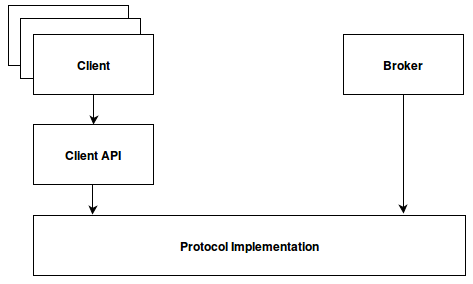
\includegraphics[width=0.55\textwidth]{images/architecture-components.png}
    \caption{Separation of code}
    \label{fig:architecture-components.png}
\end{figure}

\subsection{Consumption Model}
TODO: All requests are initiated by the client, and result in a corresponding
response message from the server

\subsection{Broker Layering}
We decided to divide the broker server application into three subsystems to
clarify the program flow from receiving data from network to handling the
requests and accessing the message log. 
\subsubsection{Network Layer}

TODO: introduction to tasks of networking layer, then ref to socket server implementation

\begin{figure}[H]
    \centering
    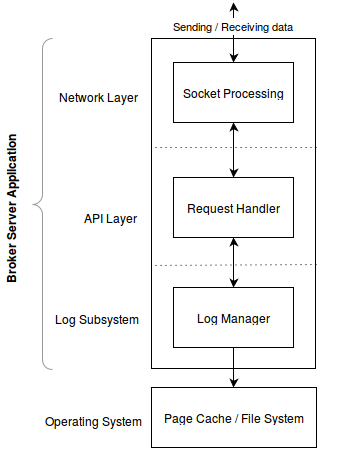
\includegraphics[width=0.3\textwidth]{images/design-subsystems.png}
    \caption{Three subsystems of broker server application}
    \label{fig:architecture-subsystems.png}
\end{figure}

\subsubsection{API Layer}

TODO: introduction to tasks of api layer, then ref to request and error handling

\subsubsection{Log}

TODO: introduction to tasks of log subsystem, then ref to persistance section



